\chapter{Broadcast}
Chiariamo con un esempio i concetti fin qui espressi. Considera un sistema
informatico distribuito in cui un'entità ha alcune informazioni importanti
sconosciute agli altri e vorrebbe condividerle con tutti gli altri. Questo
problema si chiama \textbf{broadcasting} e fa parte di una classe generale di
problemi chiamati \textbf{diffusione dell'informazione}. Risolvere questo
problema significa progettare un insieme di regole che, una volta eseguite dalle
entità, porteranno (entro un tempo finito) a tutte le entità a conoscere le
informazioni; la soluzione deve funzionare indipendentemente da quale entità
aveva le informazioni all'inizio.

Quindi:
\begin{itemize}
    \item $P_{INIT}$ = ``Solo un'entità ha l'informazione $I$ al tempo $t=0$'':
          \begin{center}
              $(\exists x \in \xi : \textrm{value}_t(x) = I) ~~ \wedge ~~ (\forall y
                  \neq x \in \xi,~\textrm{value}_t(y) = \emptyset)$
          \end{center}
    \item $P_{FINAL}$ = ``Tutte le entità hanno l'informazione $I$ al tempo $t$'':
          \begin{center}
              $\forall x \in \xi : \textrm{value}_t(x) = I$
          \end{center}
\end{itemize}

\textbf{Quindi}: Un'entità si sveglia tramite impulso spontaneo, ha
un'informazione non conosciuta dalla altre e vuole informarle tutte.

\section{Restrizioni}
Sia $\xi$ l'insieme delle entità e $G$ la topologia di comunicazione.\\
L'insieme delle restrizioni $R$ è così composto:
\begin{itemize}
    \item \colorbox{yellow}{Link bidirezionali:} grafo non orientato;
    \item \colorbox{yellow}{Affidabilità totale:} non consideriamo guasti di link
          e/o nodi;
    \item \colorbox{yellow}{Connettività:} grafo connesso, e quindi tutti possono
          raggiungere tutti;
\end{itemize}

Inoltre si ha la situazione dell'\textbf{Iniziatore Unico}: una sola entità
inizialmente è attiva.

\section{Protocollo Broadcast (senza terminazione)}
L'idea è quella che \colorbox{yellow}{se un'entità ha l'informazione $I$, allora
    la trasmette a tutti i suoi vicini.} \\ Dobbiamo specificare il
\textbf{behavior} tramite la funzione:
\begin{eqnarray}
    S \times E \rightarrow A
    \nonumber
\end{eqnarray}
\begin{itemize}
    \item $S=\lbrace$ \texttt{initiator}, \texttt{idle} $\rbrace$
    \item $E=\lbrace$ \texttt{receiving}, \texttt{alarm}, \texttt{spontaneously=I}
          $\rbrace$
\end{itemize}

L'insieme A sono sostanzialmente i protocolli che vanno scritti.

$B(x)$ = set di regole (uguali per tutte le entità):
\begin{enumerate}
    \item (\texttt{initiator x i}) $\rightarrow \lbrace$ \texttt{send(I) to N(x)}
          $\rbrace$
    \item (\texttt{idle x receiving(I)}) $\rightarrow \lbrace$ \texttt{process(I),
              send(I) to N(X)} $\rbrace$
    \item (\texttt{initiator x receiving(I)}) $\rightarrow \lbrace$ \texttt{nil}
          $\rbrace$
    \item (\texttt{idle x i}) $\rightarrow \lbrace$ \texttt{nil} $\rbrace$
\end{enumerate}
dove \textbf{$i$} corrisponde agli impulsi spontanei (eventi).\\

Il protocollo non termina poiché quando un'entità riceve I la propaga sempre a
tutto il vicinato. L'obiettivo è comunque raggiunto. Non è possibile effettuare
una stima dei costi in quanto il protocollo non termina.

Per evitare questo problema le entità dovrebbero inviare una sola volta
l'informazione, per questo si introduce lo stato \textbf{done}.

\section{Protocollo Broadcast (con terminazione)}
Per quanto riguarda la \textbf{terminazione}, abbiamo che: $S' = S \cup \lbrace$
\texttt{done} $\rbrace$

Nuove regole:
\begin{enumerate}
    \item (\texttt{initiator x i}) $\rightarrow \lbrace$ \texttt{send(I) to N(x);
              become(done)} $\rbrace$
    \item \texttt{idle x receiving(I)}) $\rightarrow \lbrace$ \texttt{process(I);
              become(done); send(I) to N(X)} $\rbrace$
    \item (\texttt{initiator x receiving(I)}) $\rightarrow \lbrace$ \texttt{nil}
          $\rbrace$
    \item (\texttt{idle x i}) $\rightarrow \lbrace$ \texttt{nil} $\rbrace$
    \item (\texttt{done x receiving(I)}) $\rightarrow \lbrace$ \texttt{nil}
          $\rbrace$
    \item (\texttt{done x i}) $\rightarrow \lbrace$ \texttt{nil} $\rbrace$
\end{enumerate}

(dove "became" indica il cambiamento di stato)\\

\colorbox{yellow}{L'idea è quella di inviare ai vicini l'informazione una sola
    volta}, quando questo accade, tutti quelli raggiunti da questa informazione
cambiano stato in \colorbox{yellow}{"Done"}. Così facendo la comunicazione
termina in tempo finito, ovvero quando tutte le entità diventano "Done".

\section{Complessità}
\subsection{Numero di Messaggi trasmessi}
Indipendentemente da $G$, abbiamo che ogni entità, che sia inizializzatore o no,
invia l'informazione a tutti i suoi vicini quindi il numero totale di messaggi
inviati è \textbf{due volte il numero degli archi}:
\begin{eqnarray}
    M[\texttt{Broadcast}, RI+]  \leq \sum_{x \in \varepsilon} N(x) = 2|E| = 2m
    \nonumber
\end{eqnarray}
Poiché $G$ ha link bidirezionali.

\textbf{Nota bene:} La notazione $RI+$ indica il fatto che si utilizza l'insieme
di restrizioni $R$ e si ha la versione del problema in cui si ha un unico
iniziatore $UI+$.

\section{Protocollo Flooding: Miglioramento del Broadcasts}
Nel normale protocollo di Broadcast quando un'entità con stato "Idle" riceve un
messaggio effettua il broadcast a tutti i suoi vicini. Questo non è necessario
poiché, per l'assioma della Local Orientation, un'entità può distinguere tra i
suoi vicini. In particolare, quando effettua il processing di un messaggio, può
identificare da quale porta lo ha ricevuto e quindi evitare di rispedirlo su
quest'ultima.\\
L'istruzione quindi diventa:

\begin{enumerate}
    \item (\texttt{initiator x I}) $\rightarrow \lbrace$ \texttt{send(I) to N(x);
              become(done)} $\rbrace$
    \item (\texttt{idle x receiving(I)}) $\rightarrow \lbrace$ \texttt{process(I),
              become(done), send(I) to $N(X) -$ {sender}}$\rbrace$
    \item (\texttt{initiator x receiving(I)}) $\rightarrow \lbrace$ \texttt{nil}
          $\rbrace$
    \item (\texttt{idle x i}) $\rightarrow \lbrace$ \texttt{nil} $\rbrace$
    \item (\texttt{done x receiving(I)}) $\rightarrow \lbrace$ \texttt{nil}
          $\rbrace$
    \item (\texttt{done x i}) $\rightarrow \lbrace$ \texttt{nil} $\rbrace$
\end{enumerate}
Dove \textbf{sender} è il vicino che ha inviato l'informazione.\\
Con questo miglioramento, tutti risparmiano un messaggio (diretto al sender)
tranne l'initiator:
\begin{center}
    $M[$\texttt{Flooding}] = $2m-n+1=O(m)$
\end{center}

\underline{Tempo:}
Chiaramente il messaggio contenente l'informazione I deve necessariamente
raggiungere anche l'entità più lontana dall'iniziatore, quindi il costo del
tempo è dato dall'\textbf{eccentricità dell'iniziatore}.
\begin{center}
    $T[$\texttt{Flooding}$, RI+] \geq \max \lbrace d(x,y) : x, y \in \xi \rbrace =
        d$
\end{center}
dove: $d$ è il diametro del grafo, il quale può anche essere visto come:
\begin{center}
    $r(x) = \max \lbrace d(x, y) : x, y \in \xi \rbrace$
\end{center}
e rappresenta l'eccentricità del nodo $x$. Tra tutte le eccentricità prendiamo
quella massima in quanto non sappiamo chi è l'initiator.\\
L'eccentricità è anche detta Diametro del grafo, ovvero il più lungo cammino
minimo tra due nodi all'interno del grafo.

\subsection{Lower Bounds per il Broadcast}
\underline{Tempo:}
Ogni entità deve necessariamente ricevere l'informazione indipendentemente dalla
sua distanza dall'Initiator, quindi:

\begin{center}
    $T($ \texttt{Broadcast, RI+} $) = \Omega(d(G))$
\end{center}

Visto che nel \texttt{Flooding} avevamo un $O(d(G))$, allora siamo ottimi in
Tempo.

\begin{theorem}
    La complessità di tempo ideale del Broadcast con $RI+$ è
    $\Theta(d(G))$.
\end{theorem}

\underline{Messaggi:}

\begin{center}
    $M($ \texttt{Broadcast, RI+} $) \geq n-1 =  \Omega(n)$
\end{center}

in quanto almeno tutte le entità che non hanno l'informazione $I$ (che sono
$n-1$), devono ricevere tale informazione. Possiamo tuttavia trovare un lower
bound più accurato.

\begin{theorem}
    $M[$ \texttt{Broadcast, RI+} $] \geq m$
\end{theorem}

\begin{proof}
    Assumiamo che esista un protocollo $A$ di broadcasting che in ogni
    esecuzione, sotto $R$ e $UI$, in ogni G, utilizzi un numero di messaggi:

    \begin{center}
        \#messaggi $< m(G)$
    \end{center}

    Questo significa che esiste almeno un link in $G$ dove non vengono trasmessi
    messaggi in nessuna direzione. Consideriamo un'esecuzione di $A$ in $G$. Sia
    $e=(x, y)$ un link su cui non vengono spediti messaggi.

    \begin{figure}[H]
        \centering
        \includegraphics[width=13cm, keepaspectratio]{capitoli/broadcast/imgs/n_09}
    \end{figure}

    Da $G$ costruiamo il grafo $G'$ ottenuto rimuovendo l'arco $(x, y)$ ed
    aggiungendo il nodo $z$ e due nuovi archi $(x, z)$ e $(y, z)$. Spostiamo sui
    due archi $(x, z)$ e $(y, z)$ le porte dell'arco $e$. Assumiamo che   $z$
    non sia l'iniziatore del protocollo. Ripetiamo la \underline{stessa
        esecuzione} di $A$ su $G'$ (supponendo quindi che lo stesso ritardo di
    comunicazione avvenga, ovvero che quando x riceveva un messaggio su G lo
    riceve nello stesso momento anche su G') per fare in modo che sia sempre lo
    stesso arco in cui non transitino messaggi. \'E possibile eseguire la stessa
    identica esecuzione di A perché nessun messaggio viene inviato sull'arco
    (x,y) (su G' nemmeno c'è questo arco).\\
    Se cosi fosse in G' nello stato finale c'è un nodo, lo $z$, che non viene
    raggiunto dall'informazione $I$, poiché negli archi che abbiamo creato non
    viene spedito nessun messaggio. Ciò è assurdo e questo implica che $A$ non è
    un protocollo di broadcasting corretto.

    \begin{center}
        $M[$ \texttt{Broadcast, RI+} $] = \Omega(m)$
    \end{center}

\end{proof}

\begin{theorem}
    Il minimo numero di messaggi richiesti dal broadcasting sotto $RI+$
    è $\Theta(m)$. \\ Il \texttt{Flooding} è \textbf{ottimo asintoticamente}.
\end{theorem}

%% vecchia parte riscritta sopra
% \theorem{ $M[$ \texttt{Broadcast, RI+} $] \geq m$
%   \begin{proof}
%     Assumiamo che esista un protocollo $A$ di broadcasting che in ogni
%     esecuzione, sotto $R$ e $UI$, in ogni G, utilizzi un numero di messaggi:
%     \begin{center}
%       \#messaggi $< m(G)$
%     \end{center}
%     Questo significa che esiste almeno un link in $G$ dove non vengono trasmessi
%     messaggi in nessuna direzione. Consideriamo un'esecuzione di $A$ in $G$. Sia
%     $e=(x, y)$ un link su cui non vengono spediti messaggi.
%     \begin{center}
%       \includegraphics[scale=0.8]{images/n_09}
%     \end{center}
%     Da $G$ costruiamo il grafo $G'$ ottenuto rimuovendo l'arco $(x, y)$ ed
%     aggiungendo il nodo $z$ e due nuovi archi $(x, z)$ e $(y, z)$. Spostiamo sui
%     due archi $(x, z)$ e $(y, z)$ le porte dell'arco $e$. Assumiamo che   $z$
%     non sia l'iniziatore del protocollo. Ripetiamo la \underline{stessa
%       esecuzione} di $A$ su $G'$ (supponendo quindi che lo stesso ritardo di
%     comunicazione avvenga, ovvero che quando x riceveva un messaggio su G lo
%     riceve nello stesso momento anche su G') per fare in modo che sia sempre lo
%     stesso arco in cui non transitino messaggi. \'E possibile eseguire la stessa
%     identica esecuzione di A perché nessun messaggio viene inviato sull'arco
%     (x,y) (su G' nemmeno c'è questo arco).\\
%     Se cosi fosse in G' nello stato finale c'è un nodo, lo $z$, che non viene
%     raggiunto dall'informazione $I$, poiché negli archi che abbiamo creato non
%     viene spedito nessun messaggio. Ciò è assurdo e questo implica che $A$ non è
%     un protocollo di broadcasting corretto.
%     \begin{center}
%       $M[$ \texttt{Broadcast, RI+} $] = \Omega(m)$
%     \end{center}
%     \fd
%   \end{proof}
% } \theorem{ Il minimo numero di messaggi richiesti dal broadcasting sotto $RI+$
%   è $\Theta(m)$. \\ Il \texttt{Flooding} è \textbf{ottimo asintoticamente}. }

\section{Broadcast su grafi particolari}

\subsection{Alberi}
Se $G$ è un albero, allora $m=n-1$.

\begin{center}
    $M[$ \texttt{Flooding, RI+} $] = 2m -n+1 = 2(n-1) -n+1 =  2n-2-n+1 = n-1 =
        O(n)$
\end{center}

Possiamo considerare il lower bound $\Omega(n)$: \texttt{Flooding} è ottimo.

\subsection{Grafi completi}
Se $G$ è un grafo completo, allora $m = \frac{n(n-1)}{2} = O(n^2)$.

\begin{center}
    $M[$ \texttt{Flooding, RI+} $] = 2m-n+1 = O(n^2)$

    $T[$ \texttt{Flooding, RI+} $] = d = O(1)$
\end{center}

Considerando il lower bound $\Omega(n)$ allora Flooding \textbf{non} è ottimo.

Nel caso in cui $G$ sia completo, possiamo progettare un algoritmo
(\texttt{KBcast}) ottimo in cui l'initiator, semplicemente, manda un messaggio
ai suoi vicini che sono $n-1$, ottenendo quindi i seguenti costi:
\begin{center}
    $M[$ \texttt{KBcast, RI+} $] = n-1$

    $T[$ \texttt{KBcast, RI+} $] = 1$
\end{center}

In pratica abbiamo messo a NIL questa istruzione: \texttt{idle x, receiving(I)}

\subsection{Ipercubi}
\begin{itemize}
    \item Un Ipercubo Orientato $H_1$ di dimensione $k=1$ è una coppia di nodi
          chiamati in binario 0 ed 1 connessi da un singolo arco la cui porta è 1 in
          entrambe le parti. Da notare che K è anche il valore nel pedice dell' H,
          quindi è sia i numeri di porta sia nel pedice.
    \item Un Ipercubo Orientato $H_k$ è ottenuto connettendo i due ipercubi di
          dimensione $k-1$ chiamati $H'_{k-1}$ e $H''_{k-1}$ e collegando i nodi con lo
          stesso nome con un link di etichetta $k$ in entrambi i nodi. Quando si va a
          creare un nuovo Ipercubo, si aggiunge uno 0 davanti alle etichette
          dell'Ipercubo già presente e in quello nuovo creato si aggiunge un 1 davanti.
\end{itemize}

\begin{itemize}
    \item $H_1$: Due nodi collegati tra di loro.
          \begin{center}
              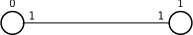
\includegraphics[scale=0.8]{capitoli/broadcast/imgs/n_10}
          \end{center}
          Come etichetta ai link si mette la dimensione dell'ipercubo.

    \item $H_2$
          \begin{center}
              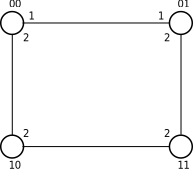
\includegraphics[scale=0.8]{capitoli/broadcast/imgs/n_11}
          \end{center}
          Due nodi adiacenti differiscono di uno ed un solo bit. Aggiungiamo un
          bit di prefisso ad ogni ``nome'' di nodo. Il valore $k$ è l'etichetta
          massima che si inserisce sugli archi. Per esempio se fossero presenti 8
          nodi, ovvero il prossimo passo della figura sopra, il k sarebbe 3,
          poiché $k = \log_2{n}$; log in base 2 di 8 fa proprio 3.
\end{itemize}

Un ipercubo di dimensione $k$ ($H_k$) avrà:
\begin{itemize}
    \item $n = 2^k$ nodi, quindi $k = \log_2{n}$;
    \item $m = n \frac{k}{2} = \frac{n}{2} \log n$ Perché ogni nodo ha $k$
          collegamenti etichettati $1,2,..,k$. Dato che abbiamo archi in comune viene
          $\frac{n}{2}$
\end{itemize}

Quindi, il costo del \texttt{Flooding} è il seguente:

$M \left[ \texttt{Flooding, RI+} \right] = 2m-n+1 =
    \cancel{2}(\frac{n}{\cancel{2}} \log n)-n+1 = n(\log n -1) +1 = n(\log n -\log
    2) +1 = n\log{\frac{n}{2}}+1 = O(n \log n)$

Possiamo vedere che il costo del \texttt{Flooding} su ipercubi non è $O(n)$ e
quindi non siamo ottimi. Vediamo ora un miglioramento di tale algoritmo adatto a
questo tipo di reti.

\subsubsection{Protocollo Hyperflood}
Il funzionamento è il seguente:
\begin{enumerate}
    \item l'initiator manda il messaggio a tutti i suoi vicini;
    \item un nodo che riceve il messaggio da un link etichettato con $l$, manda il
          messaggio soltanto ai vicini con $l' < l$.
\end{enumerate}
L'unica differenza tra HyperFlood e il normale Flooding è nel passaggio 2:
invece di inviare il messaggio a tutti i vicini tranne il mittente, l'entità lo
inoltrerà solo ad alcuni di essi, che dipenderanno dall'etichetta della porta da
cui il messaggio viene ricevuto.

\begin{lstlisting} [caption={\textit{Protocollo HyperFlood.}}]
S = {INIZIATORE, IDLE, DONE}
$S_{INIT}$ = {INIZIATORE, IDLE}
$S_{START}$ = {INIZIATORE}
$S_{TERM}$ = $S_{FINAL}$ ={DONE}

Restrictions = R

INIZIATORE
    Spontaneously
    begin
        send(m) to N(x)
        become DONE
    end

IDLE
    Receiving(M)
    begin
        LET $l$ be the port from where M arrived
        send(M) toward any $l'<l$
        become DONE
    end
\end{lstlisting}

Vedremo che questa strategia effettuerà correttamente il broadcast usando solo
$n-1$ messaggi (invece che $O(n \log n)$). Sia $H_k(x)$ il sottografo di $H_k$
indotto dai link su cui vengono spediti messaggi del protocollo HyperFlood dove
$x$ è l'iniziatore. Chiaramente ogni nodo in $H_K(x)$ riceverà l'informazione.
Bisogna dimostrare che $H_k(x)$ tocca tutti i nodi: in questo modo, il
protocollo \texttt{HyperFlood} è \textbf{corretto}.

\begin{prop}
    HyperFlood termina correttamente
\end{prop}
\begin{proof}
    %Dimostriamo che $\forall y \in \xi$ esiste un cammino da $x$, che
    %consideriamo l'iniziatore, a $y$ in $H_k$ tale che la sequenza di etichette
    %incontrate sia decrescente, ovvero 
    Bisogna provare che se all'entità y arriva un messaggio dalla porta 4,
    l'entità lo invierà solo alle porte 1,2,3. Per provare che ogni entità
    riceverà l'informazione inviata da $x$, dobbiamo mostrare che, per ogni nodo
    $y$, esiste un cammino da $x$ ad $y$ tale che la sequenza di porte
    attraversate durante il cammino è decrescente. Per effettuare questa prova
    introduciamo la seguente proprietà:
\end{proof}

\begin{prop}
    In un ipercubo $H_k$, $k$-dimensionale, ogni nodo $x$ è connesso
    ad ogni altro nodo $y$ da un cammino $\Pi \in [x,y]$ tale che la sequenza di
    etichette che si incontrano percorrendo $\Pi$ da $x$ ad $y$ è decrescente.
\end{prop}
\begin{proof}
    Consideriamo i due nodi $x,y$ dell'ipercubo $H_k$ e siano:
    \begin{center}
        $<x_k, x_{k-1}, \ldots, x_1,x_0>$ $<y_k, y_{k-1}, \ldots, y_1,y_0>$
    \end{center}
    le etichette binarie di $x$ ed $y$.

    Se $x$ e $y$ sono due nodi diversi allora il numero di bit su cui le due
    stringhe differiscono sarà:
    \begin{center}
        $t \geq 1$
    \end{center}

    Siano $j_1, j_2, \ldots, j_t$ tali posizioni in ordine decrescente, ovvero
    che $j_i > j_{i+1}$, consideriamo la sequenza di nodi:
    \begin{center}
        $v_0, v_1, \ldots ,v_t$
    \end{center}
    dove $v_0 = x$ e l'etichetta binaria del nodo $v_i$ differisce da quella di
    $v_{i+1}$ solo nella $j_{i+1}$ posizione.
    \begin{center}
        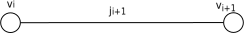
\includegraphics[scale=1]{capitoli/broadcast/imgs/n_12}
    \end{center}

    Se adesso prendo i nodi $v_0 = x $ e $v_1$, per costruzione saranno connessi
    dall'arco con etichetta $j_1$. Ma ancora per costruzione, $v_1$ sarà
    collegato a $v_2$ con l'etichetta $j_2$ e così via. Questa sequenza di nodi
    fa si che $v_t =  y$, ma questo significa che $<v_0, v_1, \ldots ,v_t>$\ è
    un cammino tra x ed y e la sequenza di etichette in questo cammino $<j_1,
        ..., j_t>$ è decrescente. Quindi $H_k(x)$ è connesso e contiene tutti i nodi
    di $H_k$ indipendentemente da $x$.\\
    In altre parole, entro un tempo finito, ogni entità avrà le informazioni.

\end{proof}

\paragraph{Costo:}

\begin{center}
    $M[$\texttt{HyperFlood}$ / H_k] = n - 1$\\
    %$T[$\texttt{HyperFlood}$ / H_k] = k = \log (n) $
\end{center}

\paragraph{Dimostrazione del Bound per i messaggi:}
Per provare che solo $n-1$ messaggi vengano inviati durante il broadcast
\textbf{bisogna mostrare che ogni entità riceverà l'informazione solamente una
    volta.} Questo è vero perché, per ogni entità $x$, $H_k(x)$ non contiene cicli
se si utilizza il protocollo HyperFlood.\\
Per avere $M[$\texttt{HyperFlood}$ / H_k] = n -1$ dobbiamo dimostrare che
$H_k(x)$ è un albero, ovvero che non ci sono cicli
\begin{proof}
    Per induzione sulla dimensione $k$\\
    \textbf{Base [$k=1$]: }$H_1(x)$ non ha cicli, poiché sono solo 2 nodi connessi
    fra di loro \\
    \textbf{Induzione: } Supponiamo vero per $H_{k-1}(x)$ e supponiamo vero anche
    per $H_k(x)$ \\
    Supponiamo quindi che $x$ sia l'iniziatore del protocollo, per come lo abbiamo
    definito, invierà un messaggio a tutti i suoi vicini $1, 2, ..., k$.
    \begin{itemize}
        \item In $H_{k-1}(x)$ ha lo stesso comportamento di un ipercubo di
              dimensione $k-1$, ma questo per induzione non conteneva cicli.
        \item Sia $y$ l'entità che è dall'altra parte dell'arco con etichetta $k$,
              il discorso vale anche per lei, per induzione.
        \item  $H_{k}(x)$ è formato da due grafi aciclici connessi da un singolo
              arco, che quindi è a sua volta aciclico.
    \end{itemize}

    Costruiamo $H_k(x)$ e rimuoviamo l'arco k-esimo dall'iniziatore, avremo quindi
    due $H_{k-1}(x)$ separati, per che ipotesi induttiva non avevano cicli.\\
    Ma allora neanche $H_k(x)$ può averne poiché per crearlo ho aggiunto un unico
    arco per unire due alberi.
\end{proof}

\textbf{Costo del Tempo:}\\
Il diametro di un Ipercubo è proprio $k$, infatti per qualunque coppia di nodi
esiste sempre un cammino con etichette decrescenti tra i due nodi, e la
lunghezza di questa commino è al più $k$.
\begin{center}
    $T[$\texttt{HyperFlood}$ / H_k] = k = \log(n) $
\end{center}
$k=\log(n)$ perché abbiamo dimostrato che $H_k(x)$ è un albero.


\begin{prop}
    Il tempo ideale necessario per il broadcasting su ipercubi
    $k$-dimensionali sotto RI+ è $\Theta(k)$.
\end{prop}

Poiché $\Omega$ del broadcasting è il diametro che in un ipercubo è $k$.

\begin{prop}
    Il numero di messaggi necessari per il broadcasting su ipercubi
    $k$-dimensionali sotto RI+ è $\Theta(n)$.
\end{prop}